\chapter{System Design}
\section{System Architecture}
The system comprises a React browser interface, a FastAPI service, a background worker, and a Python experiment engine backed by file storage. Official runs are started from the command line; custom jobs are submitted through the API and executed by the worker.
\begin{figure}[H]
\centering
\resizebox{\textwidth}{!}{%
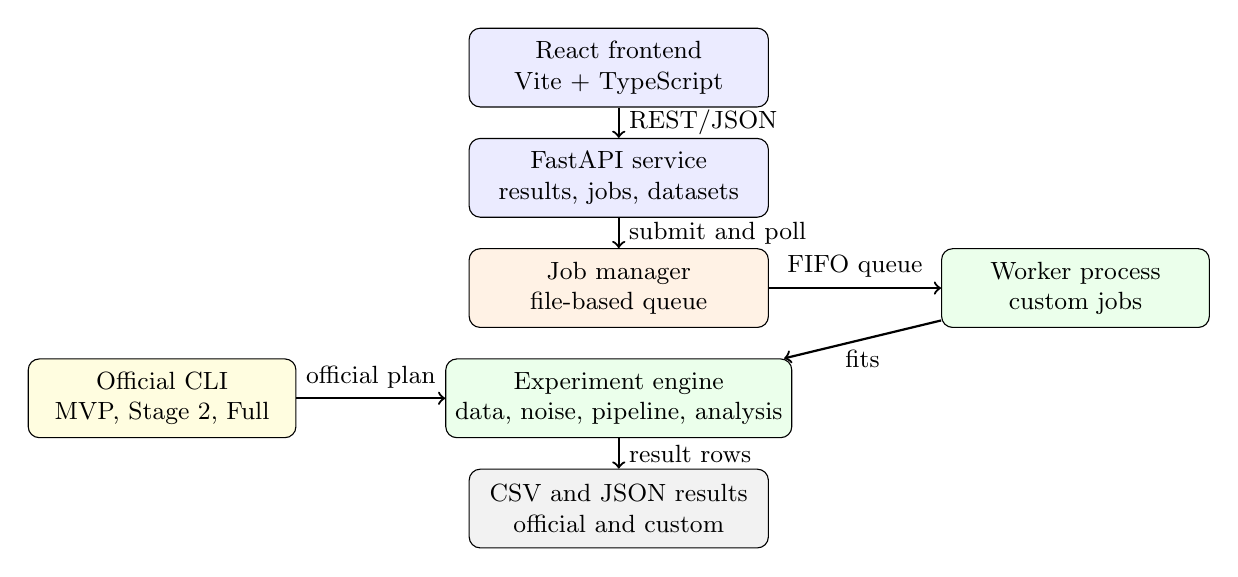
\begin{tikzpicture}[font=\small]
\node[draw, rounded corners, fill=blue!8, minimum width=3.8cm, minimum height=1.0cm, align=center] (ui) at (0,5.6) {React frontend\\Vite + TypeScript};
\node[draw, rounded corners, fill=blue!8, minimum width=3.8cm, minimum height=1.0cm, align=center] (api) at (0,4.2) {FastAPI service\\results, jobs, datasets};
\node[draw, rounded corners, fill=orange!10, minimum width=3.8cm, minimum height=1.0cm, align=center] (jobs) at (0,2.8) {Job manager\\file-based queue};
\node[draw, rounded corners, fill=green!8, minimum width=3.8cm, minimum height=1.0cm, align=center] (engine) at (0,1.4) {Experiment engine\\data, noise, pipeline, analysis};
\node[draw, rounded corners, fill=gray!10, minimum width=3.8cm, minimum height=1.0cm, align=center] (store) at (0,0.0) {CSV and JSON results\\official and custom};
\node[draw, rounded corners, fill=green!8, minimum width=3.4cm, minimum height=1.0cm, align=center] (worker) at (5.8,2.8) {Worker process\\custom jobs};
\node[draw, rounded corners, fill=yellow!12, minimum width=3.4cm, minimum height=1.0cm, align=center] (cli) at (-5.8,1.4) {Official CLI\\MVP, Stage 2, Full};

\draw[->, thick] (ui) -- node[right]{REST/JSON} (api);
\draw[->, thick] (api) -- node[right]{submit and poll} (jobs);
\draw[->, thick] (jobs) -- node[above]{FIFO queue} (worker);
\draw[->, thick] (worker) -- node[below]{fits} (engine);
\draw[->, thick] (cli) -- node[above]{official plan} (engine);
\draw[->, thick] (engine) -- node[right]{result rows} (store);
\end{tikzpicture}}
\caption{High-level system architecture. Official experiments are started from the command line; custom experiments are queued through the API and executed by a separate worker process.}
\label{fig:architecture}
\end{figure}
\section{System Workflow}
For official experiments, the engine loads the datasets and frozen configuration, splits the data, applies training-only corruption, fits each pipeline, and saves metrics and provenance. A separate analysis step produces the benchmark summaries and figures. Custom experiments follow the same approach but are queued through the API.
\section{Use Cases}
A viewer explores results and visualisations. A researcher can select a built-in dataset, use the Covertype preset, or register a CSV and specify its target column before starting a custom run. Official experiments are launched through the command line. The worker processes queued jobs and records their status.
\section{Data Flow}
Dataset and configuration inputs pass through splitting, noise injection, imputation, standardisation and classification. Predictions on the clean test split produce Macro F1 and accuracy. Raw rows feed the baseline, breaking-point, robustness and synergy analyses, which are exposed through the API to the interface.
\section{Data Storage}
The implementation uses files rather than a relational database. Raw results are stored as CSV rows, while manifests, job status and configuration use JSON. Derived CSV files contain summaries, baselines, breaking points, synergy and robustness; hashes and manifests record provenance. JSON writes are atomic and failed fits are recorded.
\section{Module Description}
The data and noise modules prepare inputs; pipeline and runner modules fit models; metrics and analysis modules compute results; storage and figure modules persist and visualise them. The API, worker and frontend connect this engine to the user.
